\documentclass{article}
\usepackage{graphicx}
\usepackage{hyperref}
\usepackage{geometry}
\usepackage{tikz}
\usepackage{tabularx}
\usetikzlibrary{positioning, arrows.meta}
 \geometry{
 a4paper,
 total={170mm,257mm},
 left=20mm,
 top=20mm,
 }

\title{Discovery Agent: Mid-term Project Report}
\author{Thue T}
\date{\today}

\begin{document}

\maketitle

\begin{abstract}
This report summarizes the progress on the Discovery Agent project, a system for automatically finding and structuring information about Danish industrial companies. It covers the research into data sources, orchestration tools, and AI API integration, and outlines the next steps for the project.
\end{abstract}

\tableofcontents

\section{Introduction}

The primary goal of this project is to create a "Discovery Agent" that can build a database of Danish industrial companies, with a focus on steel and pipe fabricators. The agent will automatically discover companies, extract their capabilities, and store the information in a structured format.

The agent will follow a cyclical process to discover and process information, as illustrated in Figure \ref{fig:workflow}.

\begin{figure}[h]
\centering
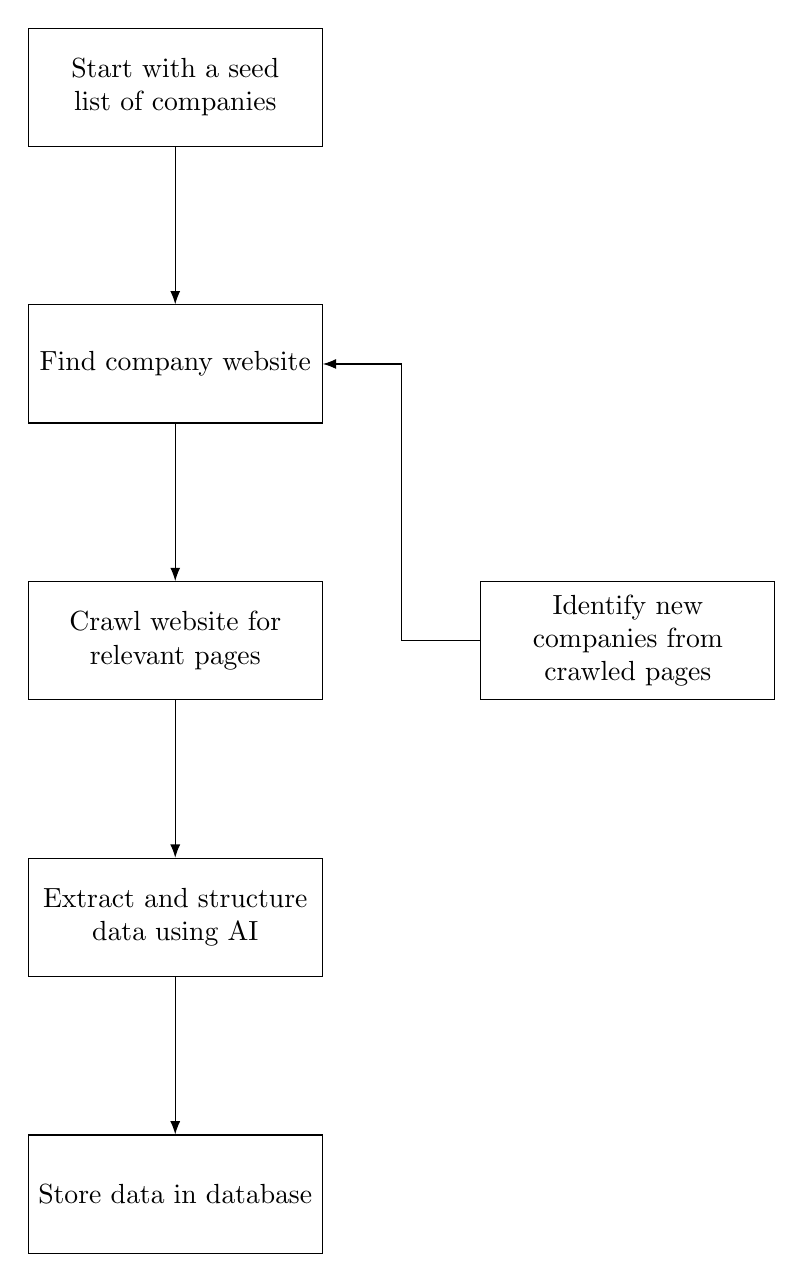
\begin{tikzpicture}[
    node distance=2cm,
    every node/.style={
        draw,
        rectangle,
        text width=3.5cm,
        text centered,
        minimum height=1.5cm
    },
    arrow/.style={-Latex}
]
    \node (start) {Start with a seed list of companies};
    \node (find) [below=of start] {Find company website};
    \node (crawl) [below=of find] {Crawl website for relevant pages};
    \node (extract) [below=of crawl] {Extract and structure data using AI};
    \node (store) [below=of extract] {Store data in database};
    \node (identify) [right=2cm of crawl] {Identify new companies from crawled pages};

    \draw[arrow] (start) -- (find);
    \draw[arrow] (find) -- (crawl);
    \draw[arrow] (crawl) -- (extract);
    \draw[arrow] (extract) -- (store);
    \draw[arrow] (identify.west) -- ++(-1,0) |- (find);

\end{tikzpicture}
\caption{Discovery Agent Workflow}
\label{fig:workflow}
\end{figure}


\section{Data Sources}

A successful Discovery Agent relies on a variety of data sources. The following sources have been identified, ranked by their usefulness for this project.

\begin{enumerate}
    \item \textbf{Official Business Registries (CVR):} The most reliable source for basic company information.
    \item \textbf{Industry-Specific Portals \& Directories:} High-value targets for finding companies in a specific sector.
    \item \textbf{Company Websites:} The primary source for detailed manufacturing capabilities.
    \item \textbf{Google Maps/Business Listings:} Good for finding locations and basic contact info.
    \item \textbf{LinkedIn:} Useful for company size and focus.
\end{enumerate}

\subsection{Accessing the Danish Business Register (CVR)}

The \textbf{CVR (Central Business Register)} is the official source of company information in Denmark. While a free official API exists, it can be complex to use. For ease of integration, a \textbf{third-party CVR API} is the recommended approach.

\subsection{Legal Considerations: GDPR}

Web scraping in the EU is subject to the \textbf{General Data Protection Regulation (GDPR)}. To minimize legal risks, the following guidelines should be followed:

\begin{itemize}
    \item Focus on non-personal company data.
    \item Avoid collecting and storing information about specific employees.
    \item Always check the terms of service of the websites you are scraping.
    \item It is strongly advised to consult with a legal professional before starting any large-scale scraping project.
\end{itemize}


\section{Workflow Orchestration}

The Discovery Agent requires a tool to orchestrate the workflow (receiving requests, making API calls, etc.). We researched several self-hosted options suitable for a TrueNAS home server.

\begin{table}[h]
\centering
\begin{tabularx}{\textwidth}{|l|l|l|l|X|}
\hline
\textbf{Tool} & \textbf{Installation} & \textbf{Resource Usage} & \textbf{Learning Curve} & \textbf{AI Orchestration Capability} \\
\hline
\textbf{n8n} & Medium & Medium-High & Medium & Excellent (built-in nodes) \\
\hline
\textbf{Node-RED} & \textbf{Low} & \textbf{Very Low} & \textbf{Low} & Good (requires custom nodes) \\
\hline
\textbf{Activepieces} & Low & Low & Low & Good (growing library) \\
\hline
\textbf{Express/FastAPI} & Low (devs) & Very Low & Low (devs) & Excellent (custom code) \\
\hline
\end{tabularx}
\caption{Comparison of Workflow Orchestration Tools}
\label{tab:orchestration_tools_comparison}
\end{table}


\subsection{Recommendation: Node-RED}

While n8n is a powerful tool, it may be overkill for this specific use case. \textbf{Node-RED is the recommended choice} for its simplicity, extremely low resource usage, and ease of setup. It provides all the necessary features to build the Discovery Agent's orchestration layer with minimal overhead.

\section{AI API Integration}

The core of the Discovery Agent is its ability to use AI to extract and structure data from unstructured text (like web pages). This requires orchestrating calls to multiple AI APIs in parallel for speed and resilience.

\begin{table}[h]
\centering
\begin{tabularx}{0.9\textwidth}{|l|X|X|X|}
\hline
\textbf{Feature} & \textbf{Anthropic Claude} & \textbf{Google Gemini} & \textbf{OpenAI GPT} \\
\hline
Authentication & API Key & API Key or Google OAuth & API Key \\
\hline
JSON Mode & Yes (with prompting) & \textbf{Yes (built-in)} & \textbf{Yes (built-in)} \\
\hline
Best For & High-quality text generation & Multimodality, Google integration & General purpose, reasoning \\
\hline
\end{tabularx}
\caption{AI API Provider Comparison}
\label{tab:ai_api_comparison}
\end{table}



\subsection{Recommended Strategy for AI Orchestration}

\begin{itemize}
    \item \textbf{Use Python with `asyncio`:} For any custom code, Python's `asyncio` library is perfect for making parallel API calls.
    \item \textbf{Use Official SDKs:} Always use the official Python SDKs for each AI provider.
    \item \textbf{Use JSON Mode:} To get structured, predictable data from the AI models, use the JSON mode offered by the APIs.
    \item \textbf{Implement Robust Error Handling:} Use a retry mechanism with exponential backoff for each API call.
    \item \textbf{Manage Costs:} Implement caching and set up billing alerts.
\end{itemize}


\section{Next Steps}

Based on the research conducted, the following next steps are recommended:

\begin{enumerate}
    \item \textbf{Set up the development environment:}
    \begin{itemize}
        \item Install and configure Node-RED on the TrueNAS server.
        \item Set up a local Python development environment for the agent.
    \end{itemize}
    \item \textbf{Develop the Agent Prototype:}
    \begin{itemize}
        \item Implement the CVR API integration to fetch basic company data.
        \item Develop the web scraper for company websites.
        \item Implement the AI integration for data extraction.
    \end{itemize}
    \item \textbf{Build the Backend and Frontend:}
    \begin{itemize}
        \item Develop the backend API to serve the collected data.
        \item Build the frontend search interface.
    \end{itemize}
    \item \textbf{Testing and Deployment:}
    \begin{itemize}
        \item Thoroughly test the entire system.
        \item Deploy the different components.
    \end{itemize}
\end{enumerate}



\end{document}

